\documentclass[11pt,a4paper]{article}
\usepackage[T1]{fontenc}
\usepackage[utf8]{inputenc}
\usepackage{amsmath,graphicx,booktabs,geometry}
\geometry{margin=24mm}
\graphicspath{{../poc/results/}}
\title{Rio Culm: transporte passivo, mobilidade do leito e dragagem}
\author{Prova de conceito reproduzível}
\date{}
\begin{document}
\maketitle
\section{Domínio e objetivo}
No trecho de 11 km do Culm, em Devon, comparam-se corridas pareadas com os mesmos contornos e condições iniciais. A geometria distribuída contém 1.130 nós e 2.019 triângulos. O canal principal de aproximadamente 19 m atravessa a planície inundável. O exemplo fornece cotas locais e um estado inicial. As séries de cheia foram substituídas por vazão de entrada constante de 28,32 m$^3$/s e cota de saída de 23,77 m. As entradas e a comparação com Danúbio e Rio Grande constam dos inventários em \texttt{docs/}. A escolha explora um trecho completo distribuído, sem representar a bacia inteira. Os dicionários e exemplos da versão v8p5r0 orientaram os CAS \cite{telemac}.
\section{Equações e parâmetros}
Para profundidade $h$, fundo $z_b$, superfície $\eta=h+z_b$ e velocidade média vertical $\mathbf u$, no domínio sem fontes volumétricas:
\begin{align}
\partial_t h+\nabla\cdot(h\mathbf u)&=0,\\
\partial_t(h\mathbf u)+\nabla\cdot(h\mathbf u\otimes\mathbf u)
&=-gh\nabla\eta+\nabla\cdot(h\nu\nabla\mathbf u)-\boldsymbol\tau_b/\rho .
\end{align}
Usa-se viscosidade horizontal constante $\nu=2$ m$^2$/s. Escrevendo $\boldsymbol\tau_b=\rho c_d |\mathbf u|\mathbf u$, as leis para lâmina larga são
\[
c_d=\begin{cases}
g/C^2 &\text{Chézy, }[C]=\mathrm{m}^{1/2}/\mathrm{s},\\
g/(K^2 h^{1/3})&\text{Strickler, }[K]=\mathrm{m}^{1/3}/\mathrm{s},\\
g n^2/h^{1/3}&\text{Manning, }[n]=\mathrm{s}/\mathrm{m}^{1/3},\\
[\kappa/\ln(\max(1.001,11.036h/k_s))]^2&\text{Nikuradse, }[k_s]=\mathrm{m}.
\end{cases}
\]
A PoC usa Strickler $K=30$. A tensão diagnóstica usa $\rho=1000$ kg/m$^3$ e valor zero para nós secos. Para concentração normalizada $c$,
\[
\partial_t(hc)+\nabla\cdot(h\mathbf u c)=\nabla\cdot(hD\nabla c).
\]
Injeta-se $c=1$ na entrada a partir de $c=0$, com $D=0,5$ m$^2$/s. Não há termo em $c$ na quantidade de movimento ou na rugosidade. Usa-se esquema N por aresta (14) no transporte advectivo para a comparação conservativa com molhamento e secagem. T2D usa elementos triangulares lineares, implicitação unitária, passo de 2 s, correção de continuidade e tratamento 2 de profundidades negativas.

Com porosidade $p=0,4$, transporte volumétrico sólido por largura $\mathbf q_b$ e remoção de volume de leito por área e tempo $d$, a evolução segue
\[
(1-p)\partial_t z_b+\nabla\cdot\mathbf q_b=-(1-p)d .
\]
GAIA usa Meyer-Peter e Müller \cite{mpm} para uma classe não coesiva de 1 mm, densidade 2.650 kg/m$^3$, sem suspensão ou aceleração morfológica. A escolha isola transporte de fundo. Com $s=\rho_s/\rho$, tensão de pele $\tau'$ e diâmetro $d_{50}$,
\[
\theta'=\frac{\tau'}{(\rho_s-\rho)g d_{50}},\quad
|q_b|=8\sqrt{(s-1)g d_{50}^3}\,[\max(\theta'-0.047,0)]^{3/2}.
\]
A correção 1 representa fundo plano e calcula a rugosidade de grão proporcional a $d_{50}$. A classe e a resistência são hipóteses exploratórias. O CLI do GAIA usa condição livre para sedimentos nas fronteiras abertas. O reuso direto do CLI hidráulico interrompeu o solver.

\section{Validação e comparações}
No primeiro ensaio, o CAS original com contornos constantes perdeu 400.111 m$^3$ no balanço acumulado. Uma tentativa de trocar o tratamento do sistema linear divergiu. A configuração final em \texttt{poc/steady.cas} manteve o tratamento 2, com tolerância do solver $10^{-8}$. Aos 54.000 s os máximos nodais de variação de $h,u,v$ nos últimos 2.000 s, divididos pelo intervalo, foram $1,11$, $3,53$ e $2,09$ vezes $10^{-6}$ em unidades SI. O critério é $10^{-5}$ para cada taxa e desequilíbrio relativo das vazões menor que $10^{-3}$. As seções de entrada e saída registraram $+28,32000$ e $-28,31967$ m$^3$/s. O critério verifica o instante escolhido para reinício, sem buscar o primeiro instante admissível.

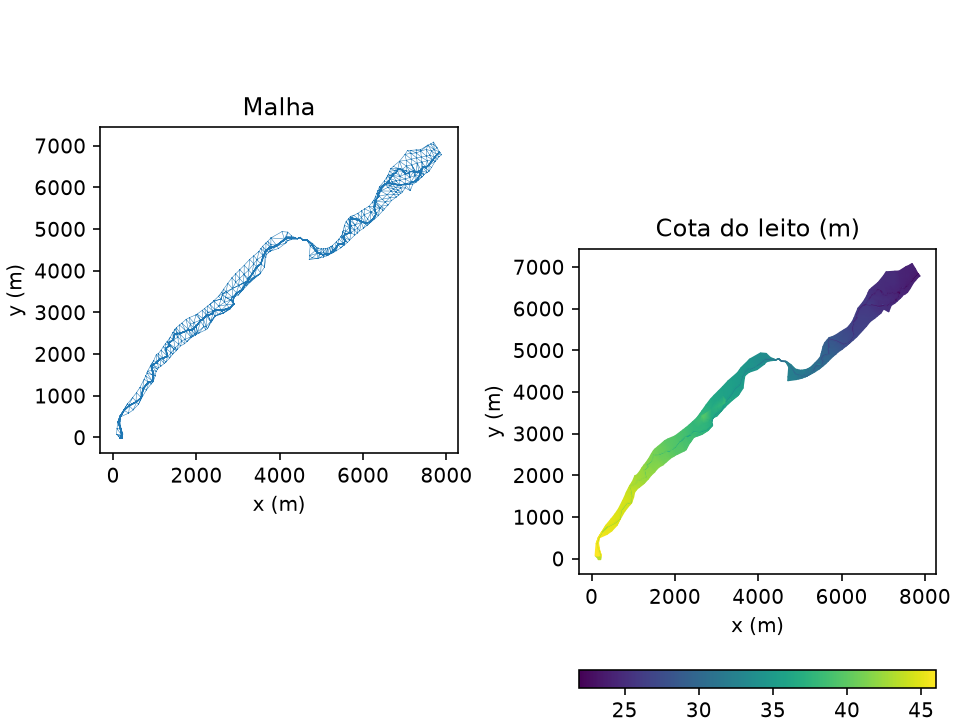
\includegraphics[width=.46\linewidth]{geometria.png}\hfill
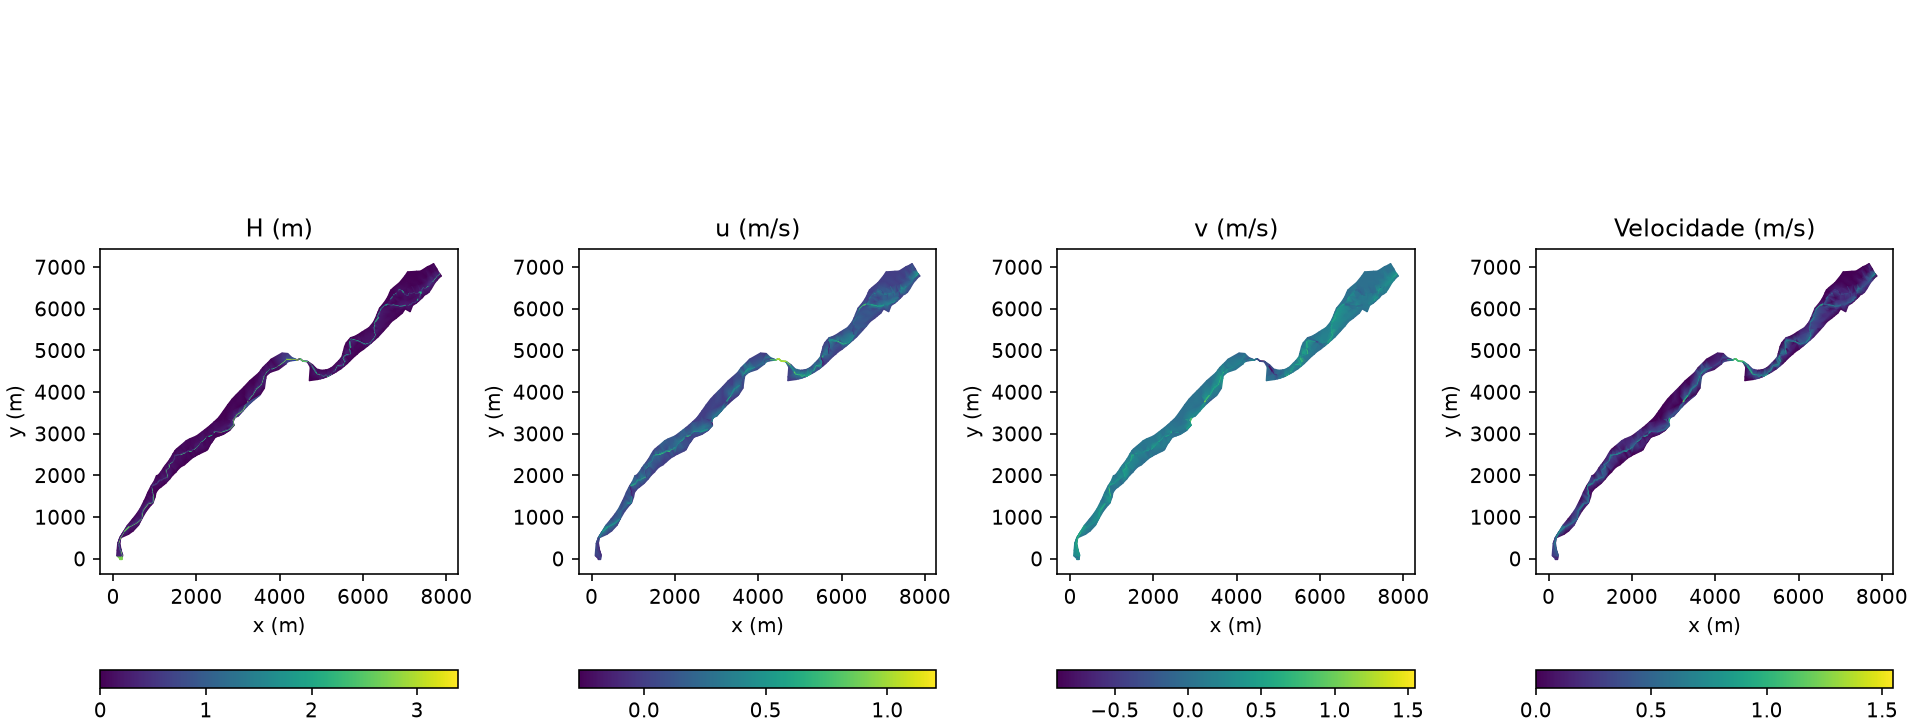
\includegraphics[width=.51\linewidth]{hidro.png}

O par com fundo fixo parte do mesmo reinício, por 1.200 s. Em seguida, cada braço continua por outros 1.200 s com GAIA. A dragagem é uma ramificação pareada nessa mesma janela morfológica. Isso controla a duração e a história hidráulica. A norma discreta $L^2=(\sum_i A_i\delta_i^2)^{1/2}$ usa um terço da área de cada triângulo incidente. As diferenças abaixo se referem ao instante final, na precisão dos Selafin.
\begin{center}
\begin{tabular}{lrr}
\toprule Comparação & Máximo absoluto & $L^2$\\\midrule
Com/sem traçador: $h,u,v,|\tau_b|$ (cada) &0&0\\
Mudança de fundo, traçador sem GAIA (m)&0&0\\
Mudança de fundo, GAIA com ou sem traçador (m)&0,02300&0,63908\\
Diferença de fundo entre os dois braços GAIA (m)&0&0\\\bottomrule
\end{tabular}
\end{center}
O balanço do traçador registrou entrada de 33.984,00 e inventário final de 35.284,57 em unidades de concentração vezes m$^3$. O resíduo relativo de $-3,69\%$ limita a interpretação quantitativa da diluição. A comparação hidrodinâmica permanece pareada. A norma integral acrescenta um fator metro às unidades do campo. A tensão foi reconstruída pela lei de Strickler. O resíduo sedimentológico acumulado do controle GAIA foi $-2,72\,10^{-4}$ kg. O Courant advectivo amostrado máximo foi 1,45, calculado com velocidade máxima dos vértices, passo de 2 s e menor altura de cada triângulo. Este diagnóstico e o balanço verificam a corrida realizada; uma análise de independência de passo ainda é necessária.

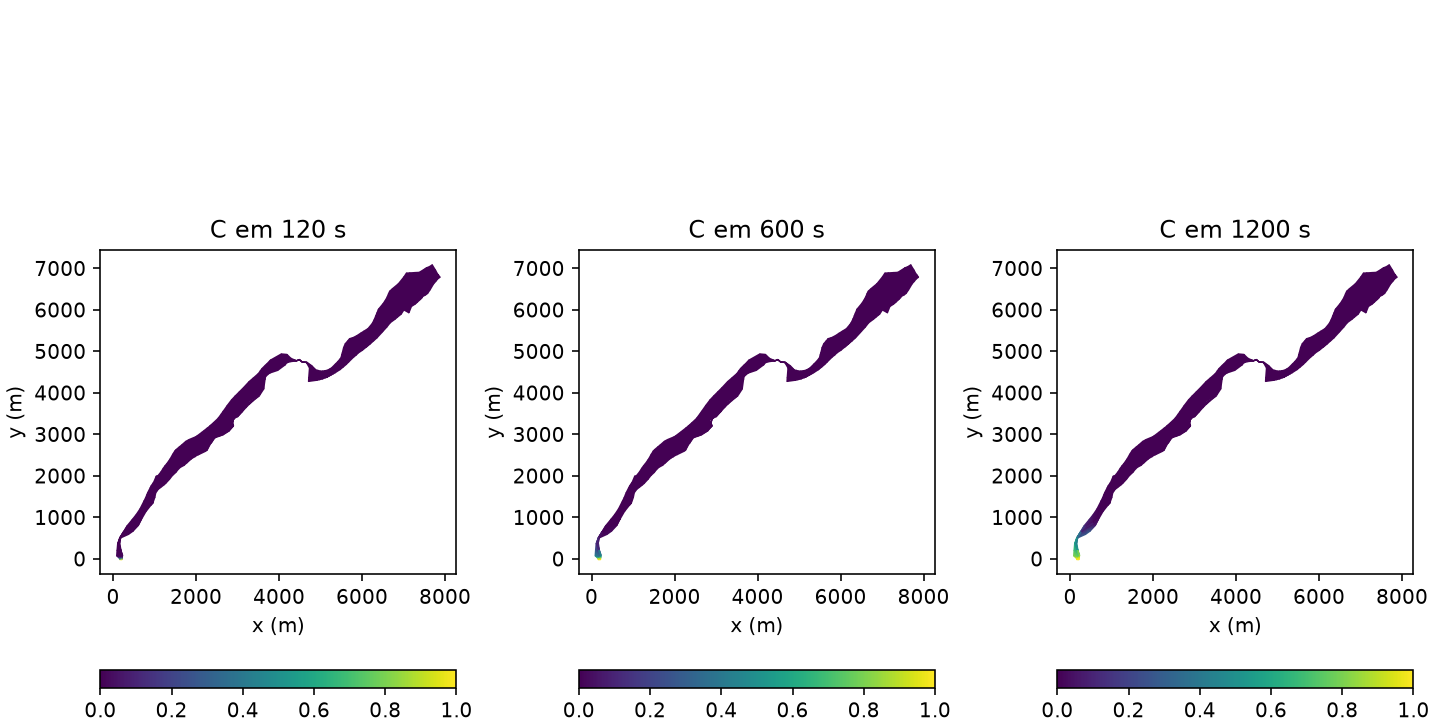
\includegraphics[width=.75\linewidth]{pluma.png}

\section{Dragagem e cortes laterais}
A instalação contém Nestor acoplado ao GAIA como alternativa ao DREDGESIM. A ação por tempo remove material do domínio entre 120 e 720 s da janela morfológica, em um quadrado de lado 170 m centrado em $(170,507)$ m. A meta é um aprofundamento médio de 0,10 m sobre a área nodal selecionada, $V=0,10\sum_{i\in P} A_i$. O solver registrou 805,918 m$^3$ removidos. As seções de referência dão a coordenada longitudinal ao diagnóstico Nestor. A execução sem esse arquivo parou no encerramento da ação.
Na comparação com traçador presente nos dois braços, a intervenção produziu máximos absolutos de 0,10008 m no fundo, 0,07316 m na profundidade, 0,07652 m/s no módulo da velocidade e 0,02107 na concentração normalizada. Os cortes interpolam os triângulos originais a $x$ fixo. A animação está em \texttt{poc/results/perfis.gif}.
\par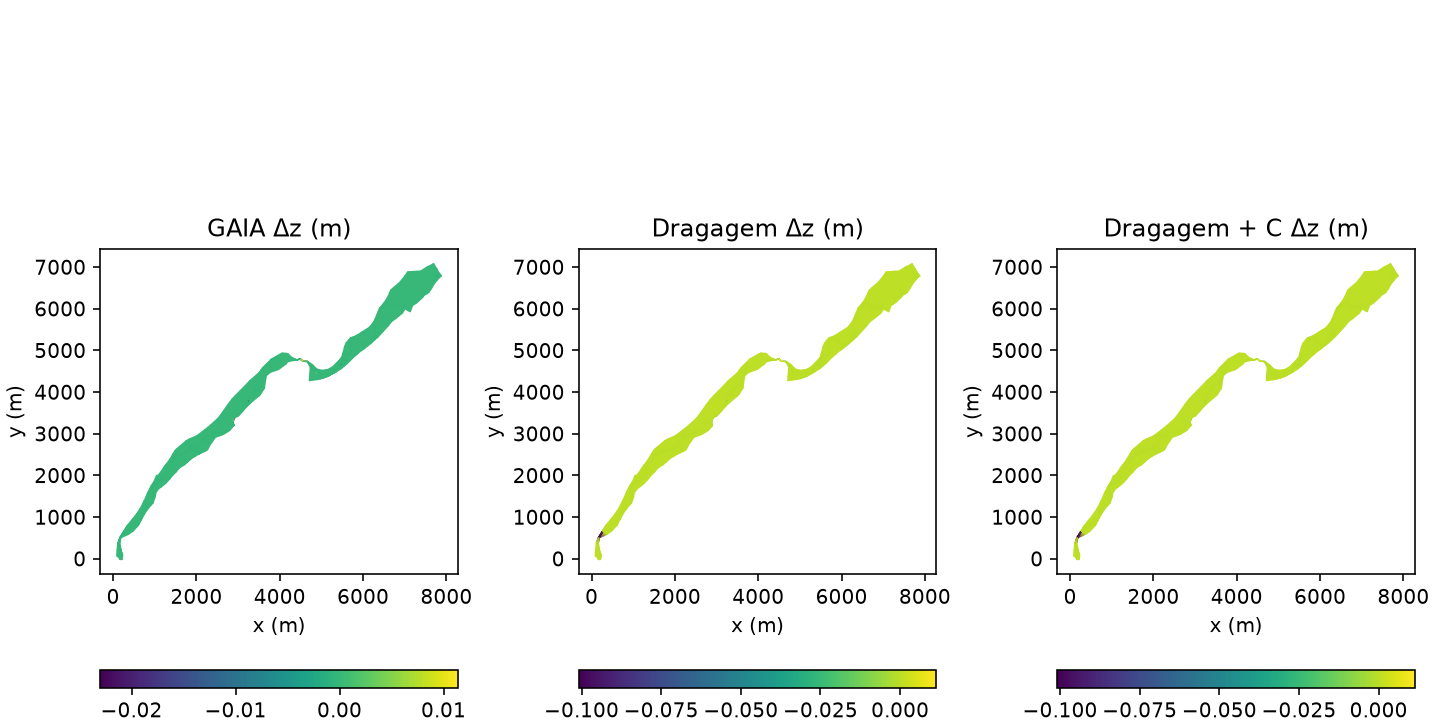
\includegraphics[width=.48\linewidth]{leito.png}\hfill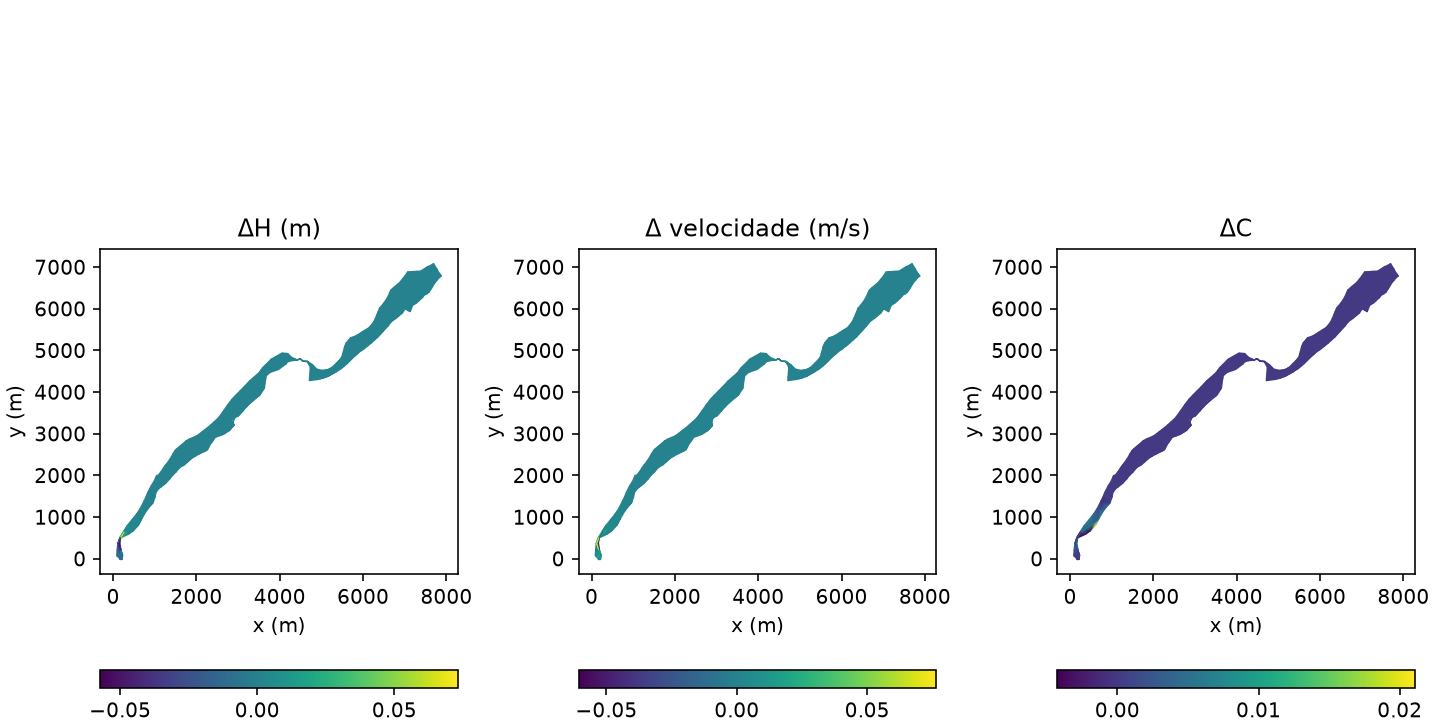
\includegraphics[width=.48\linewidth]{impacto.png}
\par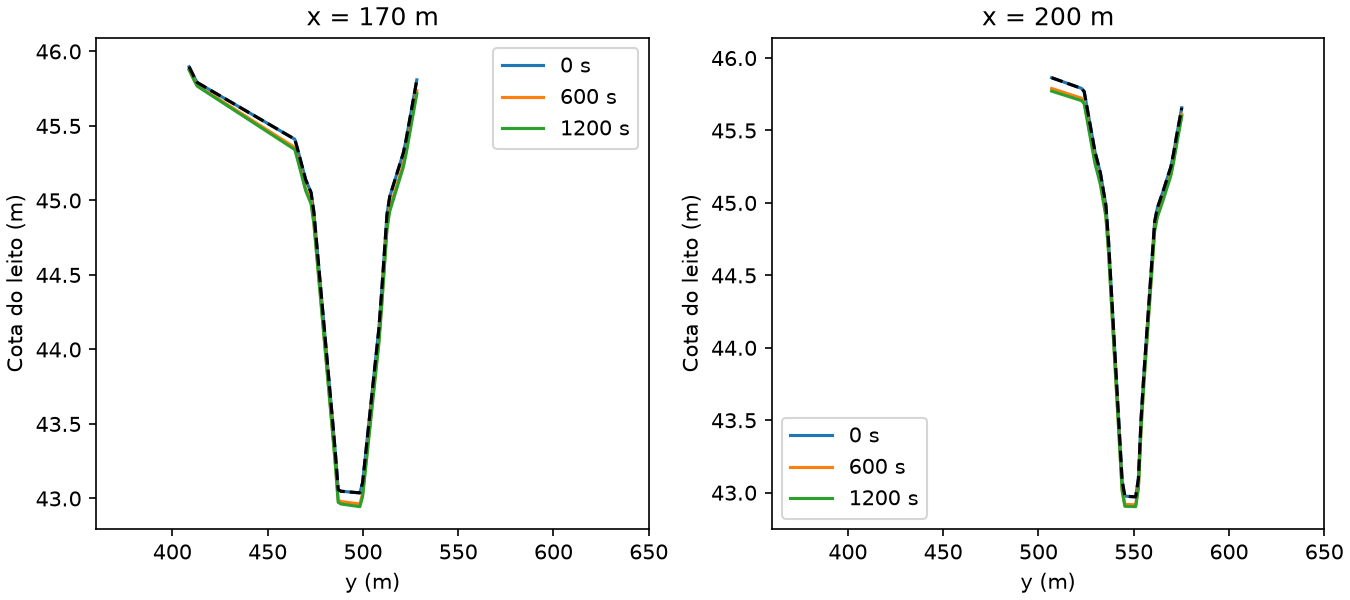
\includegraphics[width=.78\linewidth]{perfis.png}

\section{Limites e próximos ensaios}
A modelagem é promediada na vertical. Os transectos descrevem a superfície do leito. O ensaio não estima toxicidade ou transporte de metais adsorvidos. Recomenda-se ao orientador definir granulometria observada, referência vertical, polígono de projeto e tolerância de navegabilidade. A variante com retroação por densidade, a calibração da dispersão e os testes de refinamento ficam como trabalhos futuros.
\bibliographystyle{plain}
\bibliography{references}
\end{document}
